\documentclass[11pt, a4paper]{article}

\usepackage{tabularx}
%%% SST LAB PROTOCOLL PREAMBLE
%%% 2019
%%%%%%%%%%%%%%%%%%%%%%%%%%%%%%%


%%% PACKAGES
%%%%%%%%%%%%%%%%%%%%%%%%%%%

\usepackage[ngerman]{babel}

\usepackage[utf8]{inputenc}
\usepackage{amsmath}
\usepackage{pgfplots}
\usepackage{tikz}
\usepackage[many]{tcolorbox}
\usepackage{graphicx}
\graphicspath{ {./graphics/} }
\usepackage{pdfpages}
\usepackage{dashrule}
\usepackage{float}
\usepackage{siunitx}
\usepackage{trfsigns}
\usepackage{booktabs}
\usepackage[european]{circuitikz}
\usepackage{tcolorbox}

%%% DOCUMENT GEOMETRY
%%%%%%%%%%%%%%%%%%%%%%%%%%%

\usepackage{geometry}
\geometry{
 a4paper,
 total={0.6180339887498948\paperwidth,0.6180339887498948\paperheight},
 top = 0.1458980337503154\paperheight,
 bottom = 0.1458980337503154\paperheight
 }
\setlength{\jot}{0.013155617496424828\paperheight}
\linespread{1.1458980337503154}

\setlength{\parskip}{0.013155617496424828\paperheight} % paragraph spacing


%%% COLORS
%%%%%%%%%%%%%%%%%%%%%%%%%%%

\definecolor{red1}{HTML}{f38181}
\definecolor{yellow1}{HTML}{fce38a}
\definecolor{green1}{HTML}{95e1d3}
\definecolor{blue1}{HTML}{66bfbf}
\definecolor{hsblue}{HTML}{00b1db}
\definecolor{hsgrey}{HTML}{afafaf}

%%% CONSTANTS
%%%%%%%%%%%%%%%%%%%%%%%%%%%
\newlength{\smallvert}
\setlength{\smallvert}{0.0131556\paperheight}


%%% COMMANDS
%%%%%%%%%%%%%%%%%%%%%%%%%%%

% differential d
\newcommand*\dif{\mathop{}\!\mathrm{d}}

% horizontal line
\newcommand{\holine}[1]{
  	\begin{center}
	  	\noindent{\color{hsgrey}\hdashrule[0ex]{#1}{1pt}{3mm}}\\%[0.0131556\paperheight]
  	\end{center}
}

% mini section
\newcommand{\minisec}[1]{ \noindent\underline{\textit {#1} } \\}

% quick function plot
\newcommand{\plotfun}[3]{
  \vspace{0.021286\paperheight}
  \begin{center}
    \begin{tikzpicture}
      \begin{axis}[
        axis x line=center,
        axis y line=center,
        ]
        \addplot[draw=red1][domain=#2:#3]{#1};
      \end{axis}
    \end{tikzpicture}
  \end{center}
}

% box for notes
\newcommand{\notebox}[1]{

\tcbset{colback=white,colframe=green1!100!black,title=Note!,width=0.618\paperwidth,arc=0pt}

 \begin{center}
  \begin{tcolorbox}[]
   #1 
  \end{tcolorbox}
 
 \end{center} 
 
}

% box for equation
\newcommand{\eqbox}[2]{
	
	\tcbset{colback=white,colframe=green1!100!black,title=,width=#2,arc=0pt}
	
	\begin{center}
		\begin{tcolorbox}[ams align*]
				#1
		\end{tcolorbox}
		
	\end{center} 
	
}
% END OF PREAMBLE



\newcommand{\cmd}[1]{\textit{#1}}

\begin{document}


\includepdf{./titlepage/titlepage.pdf}

\section{Vorbereitungsaufgaben}
%-------------------------------------------------------------------------------
\subsection{RFC 1918}

Der RFC (Request for Comments) 1918: \emph{Address Allocation for private
 Internets} definiert die IP-Adresszuweisung für den privaten Adressbereich.
Dies erlaubt zwei Hosts gleiche IP-Adressen zu besitzen, sofern diese voneinander
isoliert sind (private Netzwerke). Zwischen beiden privaten Netzwerken stehen
dann die NAT/PAT-Devices, welche für die Übersetzung in den öffentlichen
Adressbereich und zurück sorgen.\\

Entscheidendes Kriterium ist, dass IP-Adressen, die aus dem, nach RFC 1918
definierten, privaten Adressbereich stammen auch nur in internen, privaten
Netzwerken laufen können. Das bedeutet, dass Hosts mit privaten IP-Adressen
nicht aus dem Internet erreicht werden können.\\

Es gibt 3 verschiedene Adressbereiche, welche unterschiedliche Anzahlen an Bits,
ausgehend von einer Grundadresse, für den privaten Bereich reservieren (vgl.
Netzklassen) (nicht zu verwechseln mit Subnetting).

\begin{table}[H]
 \begin{center}
\begin{tabular}{llll}
\rowcolor{teal-0}
Adressbereich                 & Blockgröße & CIDR Kennz.    & Anzahl\\
10.0.0.0 - 10.255.255.255     & 24 bit     & 10.0.0.0/8     & 16777216\\
172.16.0.0 - 172.31.255.255   & 20 bit     & 176.16.0.0/12  & 1058576\\
192.168.0.0 - 192.168.255.255 & 16 bit     & 192.168.0.0/16 & 65536
\end{tabular}
 \end{center}
\caption{RFC 1918 private Adresszuweisungen}
\end{table}

Die restlichen $2^{32}-2^{24}-2^{20}-2^{16} = 4.277.075.968$ Adressen für den
öffentlichen Bereich werden von der \textsc{IANA} (Internet Assigned Numbers
Authority) verwaltet.

%-------------------------------------------------------------------------------
\subsection{Anzahl intern local auf intern global}
PAT weist jeder TCP oder UDP Kommunikation eine einzigartige Quellportnummer zu,
was die Abbildung der Adressen mehrerer lokaler (insidel local) Geräte auf
eine einzige öffentliche (inside global) Adresse ermöglicht.\\

Da der Port eine 16-bit Zahl ist und somit maximal den Wert 65535 haben kann,
ist die maximale Anzahl dieser Zuweisungen auf eine einzige inside global IP
durch die Portnummer limitiert.\\

Hinzu kommt, dass ein Host-Gerät (einzelne inside local IP) durchaus
gleichzeitig mehrere Verbindungen mit unterschiedlichen Quellports herstellen
kann (z.B. Browser bei Öffnen einer Website). Dadurch wird die Anzahl der
mit NAT verwalteten Geräte limitiert.

%-------------------------------------------------------------------------------
\subsection{Vor- und Nachteile von NAT / PAT}

\begin{table}[H]
\begin{tabularx}{\textwidth}{|X|X|}
  \textbf{Vorteile} & \textbf{Nachteile}\\
  \hline
  $\rightarrow$ Mehrere Hosts auf eine IP-Adresse zuordenbar, dadurch werden IPv4 Adressen gespart & $\rightarrow$ Erhöhter technischer Aufwand / zusätzlicher Schritt der Übersetzung notwendig\\
  $\rightarrow$ Anonymisierung der Hosts gegenüber der outside global/local Seite &$\rightarrow$ Begrenzter Speicher des NAT-Gerätes bei hoher Anzahl an Übersetzungseinträgen\\
  $\rightarrow$ Höhere Flexibilität und Übersichtlichkeit im Network-Design & $\rightarrow$ Komplikationen bei VPN\\
  & $\rightarrow$ Router sollte eigentlich nicht auf Ebene 4 (Portnummern) agieren
\end{tabularx}
\end{table}

%-------------------------------------------------------------------------------
\subsection{Unterscheidungsmerkmale am NAT-Device}
Die Unterscheidungsmerkmale sind:

\[\{\text{Quell-IP, Quell-Port, Ziel-IP, Ziel-Port, Protokoll}\}\]\\

Das NAT-Device (i.d.R. Router) führt eine Tabelle über bestehende Verbindungen
und den zugehörigen Adress- und Portübersetzungen.\\

Ein Sonderfall bildet das ICMP-Protokoll (z.B. bei ping-Befehl), da es auf
Ebene 3 arbeitet und daher keine Portnummern verwendet. Dieser Fall wird im RFC
5508 definiert. Für ICMP-Anfrage und -Antwort Nachrichten (query/reply) legt
das NAT-Gerät, ähnlich wie bei PAT, eine Query-ID an, die den jeweiligen Host
identifiziert.\\



%-------------------------------------------------------------------------------

\section{Versuchsaufgaben}
\subsection{NAT-Untersuchung I}

Die PCs 1-4 wurden nach Versuchsanleitung mit der entsprechenden
Netzwerkkonfiguration unter Windows konfiguriert. Daraufhin wurde die
Kommunikation zum Standardgateway mittels ping-Befehl überprüft (erfolgreich).\\

Mittels Firefox-Browser wurde dann versucht, eine HTTP-Verbindung zur externen
Adresse \inlinecode{193.175.118.49} (extern global) auf jedem der 4 Rechner
herzustellen.\\

Mithilfe des \cmd{netstat}-Befehls wurden die TCP-Verbindungen jedes Rechners
nach der Eingabe der IP-Adresse in die URL-Leiste überprüft. In Abb.
\ref{PC3_netstat} erkennt man den erfolgreichen Website-Aufruf (links), welcher
durch \cmd{netstat} (rechts) mit dem Status HERGESTELLT bestätigt wird.\\

Bei PC2, sowie bei den anderen PCs konnte jedoch keine Verbindung hergestellt
werden. In Abb. \ref{PC2_netstat} kann man die Firefox-Fehlermitteilung der
unterbrochenen Verbindung sehen. Hier zeigt die \cmd{netstat}-Ausgabe drei
angefragte Verbindungen (SYN\_GESENDET) auf unterschiedlichen Quellports,
die jedoch keine Antwort erhalten.\\

\begin{figure}[H]
  \centering
  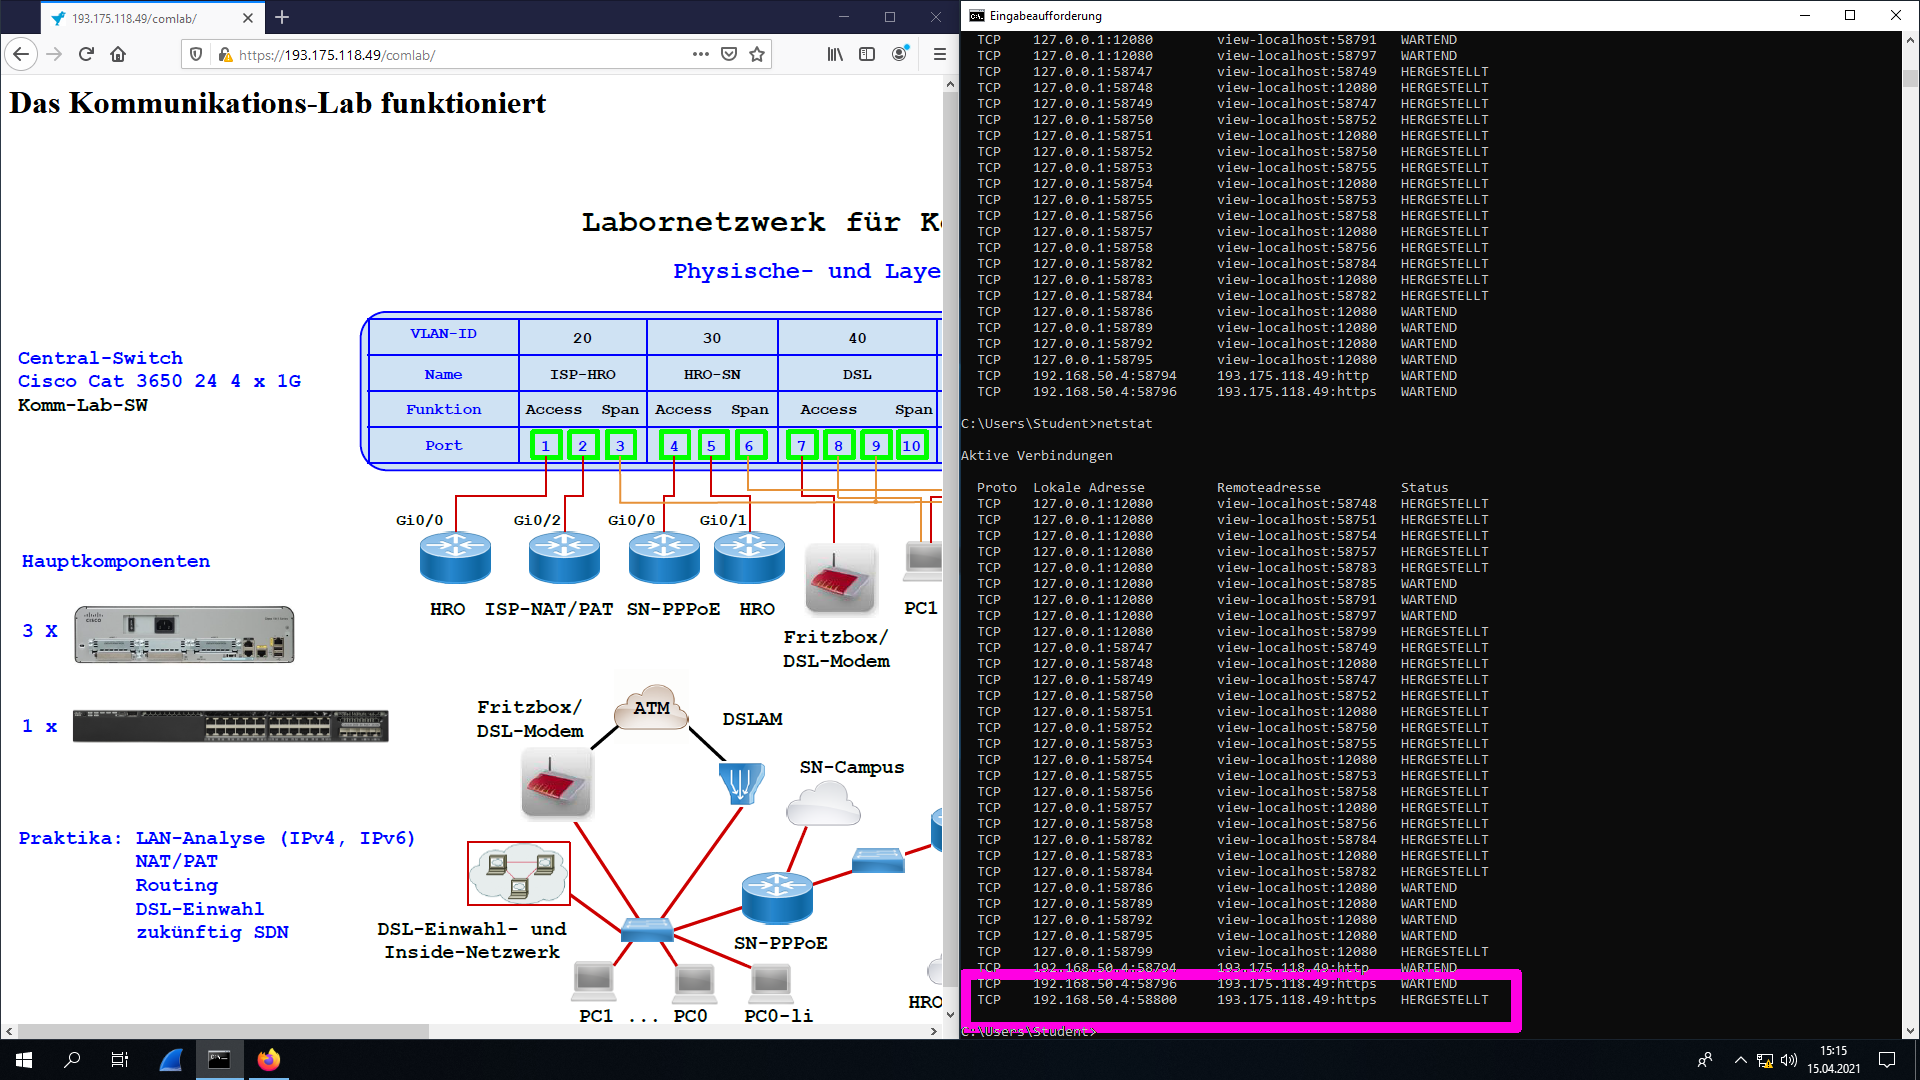
\includegraphics[width=\textwidth]
  {graphics/bilder/31/PC_3_zweiterversuch_verbunden}
  \caption{\emph{netstat} von PC3}\label{PC3_netstat}
\end{figure}

\begin{figure}[H]
  \centering
  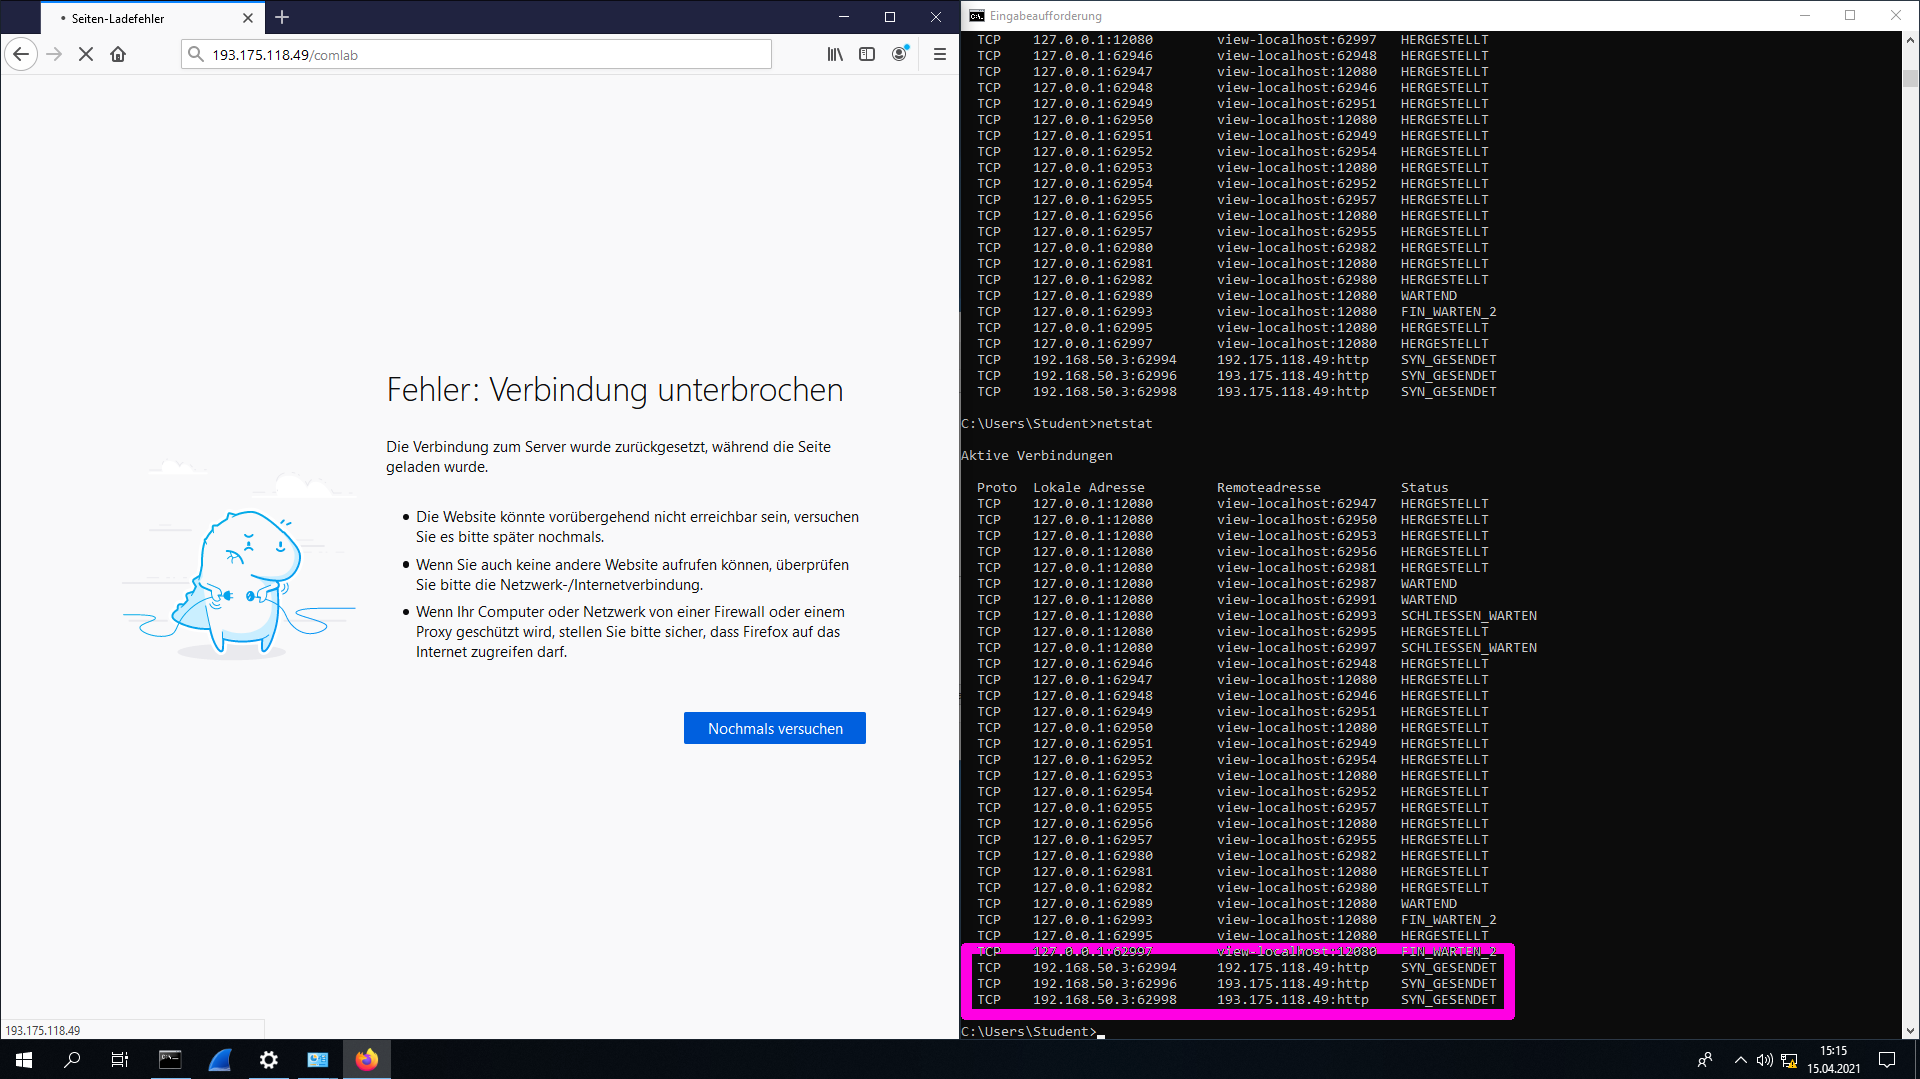
\includegraphics[width=\textwidth]
  {graphics/bilder/31/PC_2_zweiterversuch_nichtverbunden}
  \caption{\emph{netstat} von PC2}\label{PC2_netstat}
\end{figure}

Betrachtet man den Wireshark-Trace, kann man den Port 58800 wiederfinden, wie
er auch in Abb. \ref{PC3_netstat} zu sehen ist. In Abb. \ref{58800_handshake}
erkennt man den 3-way-handshake auf ebendiesem Port, hier jedoch nicht mit der
lokalen IP-Adresse aus Abb. \ref{PC3_netstat}, sondern mit der öffentlichen
Adresse \inlinecode{212.201.38.175}. Daraus lässt sich also die NAT-Übersetzung
von der inside local Adresse \inlinecode{192.168.50.4:58800} auf die inside
global Adresse \inlinecode{212.201.38.175:58800} bestimmen. Da der Port 58800
anscheinend nicht belegt war, wurde die Portnummer zudem nicht in eine
andere übersetzt.\\

Dass PC2 keine Verbindung herstellen konnte, liegt an der begrenzten Anzahl
(pool) der öffentlichen IP-Adressen, die dem NAT-Gerät zur Verfügung stehen und
die zusätzlich durch die anderen Laborteilnehmer genutzt wurden. PC2 konnte
demnach keine inside global IP-Adresse zugewiesen werden, wodurch der externe
HTTP-Server auch nie ein SYN-Paket von ihm erhalten konnte.\\

Auch der PC2-Versuch kann im Wireshark erkannt werden (Abb. \ref{why}), jedoch
konnte nicht geklärt werden, weshalb PC0 diese mitschneidet, da es aus Sicht
der gegebenen Topologie keine lokalen Pakete mitschneiden sollte.\\

\begin{figure}[H]
  \centering
  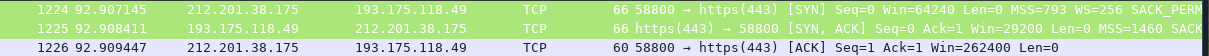
\includegraphics[width=\textwidth]
  {graphics/bilder/31/ws_58800_handshake}
  \caption{Three-Way-Handshake auf Port 58800}\label{58800_handshake}
\end{figure}

\begin{figure}[H]
  \centering
  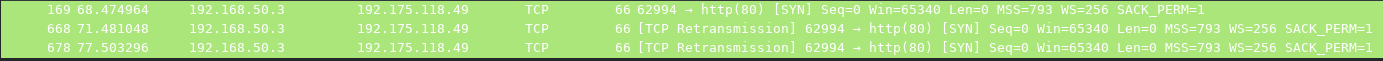
\includegraphics[width=\textwidth]
  {graphics/bilder/31/why}
  \caption{Mitschnitt der Verbindungsversuche von PC2 mit Quellport 62994.
  Es ist keine Übersetzung in eine öffentliche IP-Adresse erkennbar}\label{why}
\end{figure}

%-------------------------------------------------------------------------------

\subsection{NAT-Untersuchung II}

In der weiteren Untersuchung wurden Verbindungsversuche von einem Gerät, das
mit dem Campusnetz verbunden war an einen im Labor befindlichen HTTP-Webserver
auf PC4 getätigt.\\

Da sich beide Kommunikationspartner (Client und Server) in unterschiedlichen
privaten Netzwerken befinden, war auch hier eine NAT-Übersetzung zu erwarten.\\

\begin{figure}[H]
  \centering
  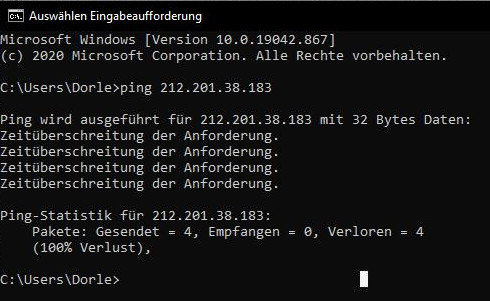
\includegraphics[width=0.618\textwidth]
  {graphics/bilder/32/ping_laptop}
  \caption{Ping-Versuch von externem Gerät}\label{ping_fail}
\end{figure}

Die inside global IP-Adresse des Servers war \inlinecode{212.201.38.183}. Auf
dem externen Gerät (Laptop) wurde versucht, diese IP-Adresse mit dem ping-
Befehl zu erreichen. Wie in Abb. \ref{ping_fail} zu sehen, ist dies gescheitert.
% Der Grund hierfür liegt darin, dass sich zwischen externem Gerät (Campusnetz)
% und dem Webserver das NAT-Gerät befindet, welches für die IP-Übersetzung
% zuständig ist. Da der Ping lediglich an die öffentliche IP-Adresse \inlinecode{
%   212.201.38.183} gerichtet war und aus Sicht des externen Gerätes sich im
% outside local Netz mehrere lokale Geräte befinden, gab es keine Möglichkeit für
% das NAT-Gerät (Router) den Server zu identifizieren und die Anfrage zuzuweisen
% (keine Portnummer, wie z.B. bei HTTP-Anfrage), weshalb sie fallengelassen wurde.\\

\begin{figure}[H]
  \centering
  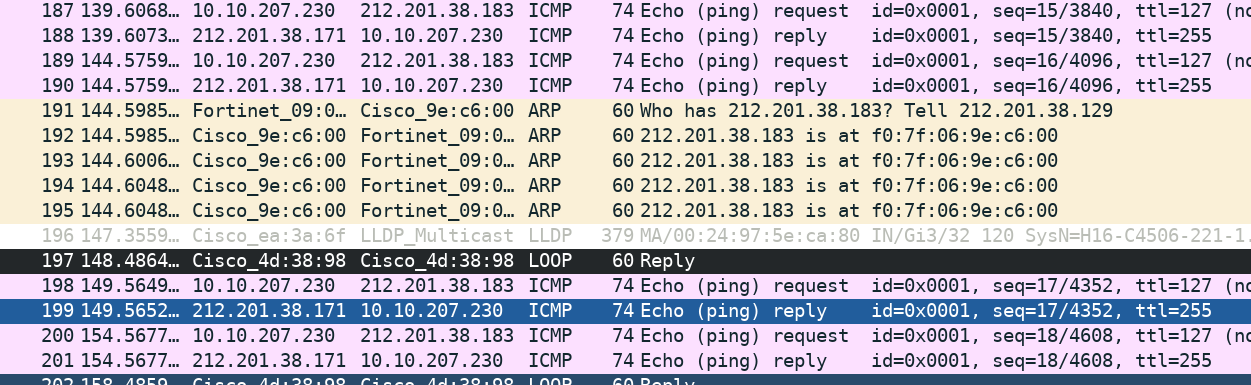
\includegraphics[width=0.618\textwidth]
  {graphics/bilder/32/ping_laptop_pc0_reply}
  \caption{Wireshark-Mitschnitt des ping-Verkehts vom externen PC and PC0}\label{ping_laptop_pc0_reply}
\end{figure}

In Abb. \ref{ping_laptop_pc0_reply} sieht man die ping-Anfragen von
\inlinecode{10.10.207.230} (Laptop) an die Adresse des Servers \inlinecode{212.201.38.183},
welche jedoch nicht von dieser sondern von der Adresse \inlinecode{212.201.38.171}
beantwortet werden. In Abb. \ref{ping_laptop_pc0_reply} erscheint dies als nichtempfangene
Antwort am Laptop, da Ziel und Empfangsquelladresse des pings nicht übereinstimmen.\\

Der Adresse \inlinecode{212.201.38.171}, von der die Antwort kam, wird auf Ebene
2 die MAC-Adresse \inlinecode{f0:7f:06:9e:c6:00} zugewiesen, welche auch mit
der MAC-Adresse hinter den TCP-Anfragen aus Aufgabe 1 übereinstimmt. Es handelt
sich dabei also um den Gateway des Labornetzes (PC1..PC4).

\begin{figure}[H]
  \centering
  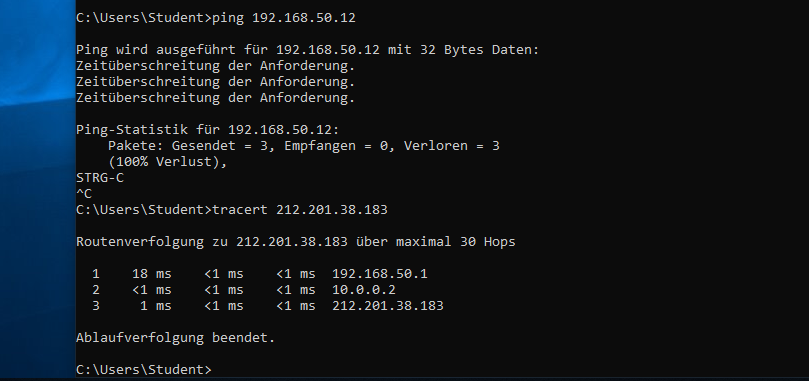
\includegraphics[width=0.618\textwidth]
  {graphics/bilder/32/32_tracrt_intern_erfolgreich}
  \caption{Ping von PC3 an PC4 (lokal)}\label{ping_internx}
\end{figure}

Auch der interne ping von PC3 an PC4 erhielt keine Antwort (Abb. \ref{ping_internx}),
was vermuten lässt, dass die Firewall an PC4 keine Ping-Anfragen durchgelassen hat.
Der Wireshark Trace an PC4 bestätigt dies, da dort während der Durchführung keine
ICMP-Pakete aufgezeichnet wurden. Wahrscheinlich wurde im externen Fall daher
auch die ICMP-Fehlermeldung vom Gateway erhalten.\\

\begin{figure}[H]
  \centering
  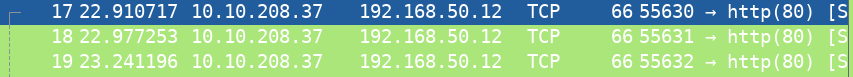
\includegraphics[width=0.618\textwidth]
  {graphics/bilder/32/bleppo}
  \caption{TCP-Verbindung an PC4}\label{ping_txcpp}
\end{figure}

Die TCP-Verbindungen wurden bei Websiteaufruf über Firefox aufgebaut, jedoch
zeigt der Wireshark-Mitschnitt in Abb. \ref{ping_txcpp} zwei lokale IP Adressen
zwischen denen die Verbindung aufgebaut wird, allerdings ist hier auch nicht
bekannt, weshalb diese erscheinen und (scheinbar) kein NAT-Mechanismus dazwischen
steht.\\

Bei der Umstellung des Webservers ist ein Fehler aufgetreten, weshalb die zweite
Seite nicht erreicht werden konnte. Einige weitere Betrachtungsweisen fehlen leider,
was der begrenzten Praktikumszeit geschuldet ist.

%-------------------------------------------------------------------------------

\subsection{NAT-Untersuchung III}
Zu Beginn wird der Domainname hermes.fiw.hs-wismar.de in eine IP-Adresse über
DNS aufgelöst. Hierbei findet man mehere Anfragen. Da DNS über UDP läuft, kann
man auch die Portnummern der Anfragen einsehen und erkennen, dass sie von
unterschiedlichen Rechnern stammen.\\

\begin{figure}[H]
  \centering
  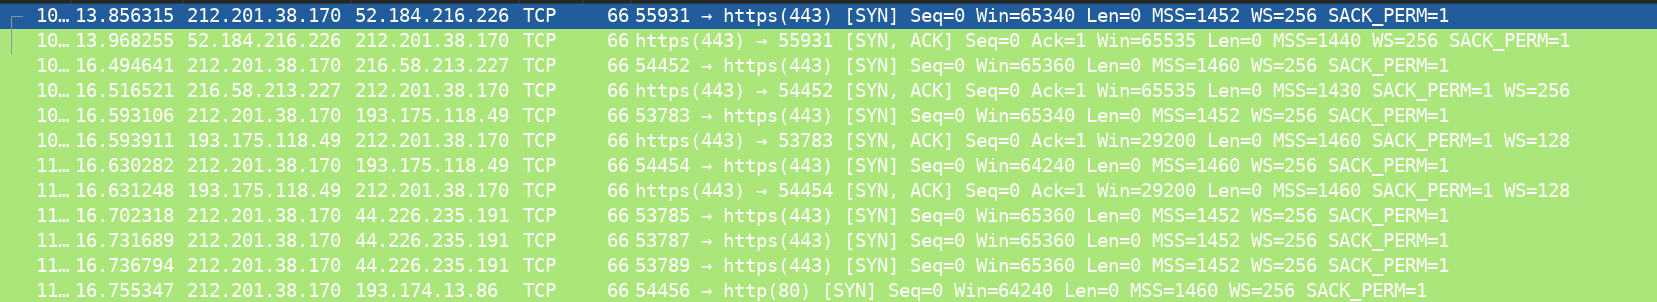
\includegraphics[width=\textwidth]
  {graphics/bilder/33/ws_total}
  \caption{Mitschnitt der SYN-Pakete von verschiedenen lokalen PCs über die gleiche
    öffentliche IP
  }\label{33_ws_total}
\end{figure}

Aus Abb. \ref{33_ws_total} lässt sich erkennen, dass mehrere HTTP-Verbindungen
über die gleiche öffentliche IP-Adresse laufen, diese sich jedoch in der
TCP-Portnummer unterscheiden. Diese Portnummern ermöglichen dem NAT-Gerät die
eindeutige Zuweisung der Hostgeräte.\\

Es kann sich hierbei nicht um statisches NAT handeln, da sonst jeder Verbindung
eine andere öffentliche IP aus einem Pool von verfügbaren IP-Adressen zugewiesen
worden wäre. Man kann daher definitiv sagen, dass es sich um dynamisches NAT
handelt. Da die inside global Portnummern jedoch mit den inside local Portnummern
übereinstimmen, kann man nicht genau sagen, ob es sich um die Sonderform PAT
handelt oder um einfaches dynamisches NAT (Abb. \ref{33_w_total}).

%-------------------------------------------------------------------------------

\subsection{Ping-Kommando}

Auszug aus dem \emph{Internet-Draft: NAT Behavioral Requirements for ICMP}:
\begin{quote}
  \textit{ICMP Query Messages - All ICMP query messages are characterized
   by the fact that have an Identifier field in the ICMP header. The
   Identifier field used by the ICMP Query messages is also referred
   as "'Query Identifier"' or "'Query Id"' for short throughout the
   document. A Query Id is used by query senders and responders as
   the equivalent of a TCP/UDP port to identify an ICMP Query session.}
 -- Internet-Draft: NAT Behavioral Requirements for ICMP, May 2006
\end{quote}

Das Feld \emph{Identifier} im Header des ICMP-Protokolls wird demnach also als
eindeutige Kennzeichnung für die ICMP-Nachrichten am NAT-Gerät verwendet und
stellt somit den Ersatz für den Schicht 4 Port dar.\\

Im Wireshark Trace der Pings der lokalen Rechner PC1 bis PC4, wie er an PC0
mitgeschnitten wurde (Abb. \ref{ws_total}) sieht man, dass alle ICMP-Anfragen
über die gleiche öffentliche IP-Adresse laufen, wie es zu erwarten war.\\

\begin{figure}[H]
  \centering
  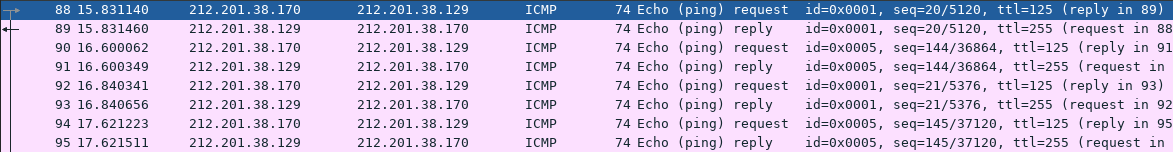
\includegraphics[width=\textwidth]
  {graphics/bilder/zusatz/ws_total}
  \caption{Mitschnitt der Ping-Anfragen von verschiedenen lokalen PCs mit an PC0
  }\label{ws_total}
\end{figure}

Schaut man sich die erste Anfrage in Wireshark genauer an (Abb. \ref{z_first_req}),
erkennt man in dessen ICMP-Header im \emph{Identifier}-Feld die Nummer 0x0001.

\begin{figure}[H]
  \centering
  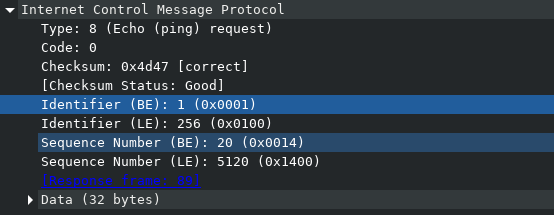
\includegraphics[width=0.618\textwidth]
  {graphics/bilder/zusatz/first_req}
  \caption{Genauere Betrachtung der ersten ICMP-Anfrage}\label{z_first_req}
\end{figure}

Bei der zweiten Anfrage (Zeile 3 in Abb. \ref{ws_total}) sieht man einen anderen Wert im Identifier-Feld, nämlich 0x0005 (Abb. \ref{z_second_req}).

\begin{figure}[H]
  \centering
  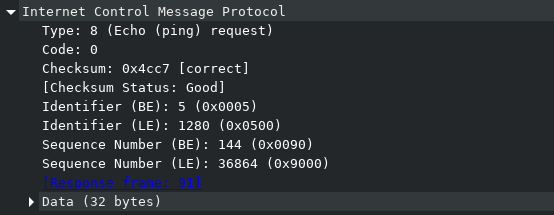
\includegraphics[width=0.618\textwidth]
  {graphics/bilder/zusatz/second_req}
  \caption{Genauere Betrachtung der zweiten ICMP-Anfrage}\label{z_second_req}
\end{figure}

Bei der dritten Anfrage (Zeile 5 in Abb. \ref{ws_total}) findet man wieder den Identifier 0x0001, wie auch bei der ersten in Abb. \ref{z_first_req} (Abb. \ref{z_third_req}). Sie ist demnach auch dem gleichen Host wie bei der ersten Anfrage zuzuordnen.

\begin{figure}[H]
  \centering
  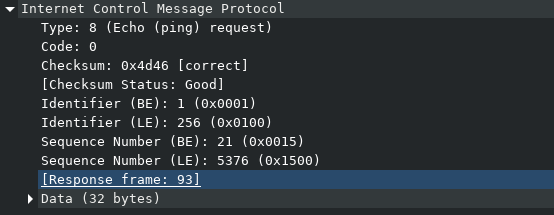
\includegraphics[width=0.618\textwidth]
  {graphics/bilder/zusatz/third_req}
  \caption{Genauere Betrachtung der dritten ICMP-Anfrage}\label{z_third_req}
\end{figure}

Die einzelnen Anfragen kommen also über die gleiche öffentliche IP-Adresse, werden aber durch ihre Identifier-Felder im ICMP-Header voneinander unterschieden, was sich mit den Erwartungen deckt.

\end{document}
